%09.10.2024, lecture 2

\section{One-way~Functions}\label{sec:one_way_functions}

Let $\fP$ denote the class of functions that can be computed in~polynomial~time.
Similarly, let $\FP$ denote the class of problems for which a~solution can be found in~polynomial~time.

\begin{definition}
	A \emph{one-way function} is an injective function that can be efficiently computed (in~polynomial~time), but whose inverse cannot be efficiently computed (in~polynomial~time).
\end{definition}

\begin{theorem}
    If $\PP \neq \NP$, then there exists an $f \in \fP$ such that $f^{-1} \not\in \fP$.
\end{theorem}

\begin{proof}
    Let $\Phi$ be a Boolean formula, and let $A \in \{0, 1\}^n$ be a Boolean assignment to its $n$ variables.
    Define
    \begin{align*}
        f(\Phi, A) = \begin{cases}
        (\Phi, 1^n), &\text{ if } \Phi[A]=1, \\
        (\Phi, 0^n), &\text{ if } \Phi[A]=0.
        \end{cases}
    \end{align*}
    If we could invert $f$, we would be able to solve SAT by computing $f^{-1}(\Phi, 1^n)$.

    Therefore, if $\PP \neq \NP$ and both $f$ and $f^{-1}$ belong to $\fP$, it would imply $\PP = \NP$.
    Conversely, if $\PP = \NP$, then $f^{-1} \not\in \fP$.
\end{proof}

\begin{exercise}
	Prove the converse of our "worst-case theorem": if there exists an $f$ such that $f \in  \fP$ and $f^{-1} \not\in \fP$, then $\PP \neq \NP$.
\end{exercise}

\begin{proof}
	Assume that $f \in  \fP$, $f^{-1} \not\in  \fP$, and that $\PP = \NP$.
	In this case, we could invert $f$ by nondeterministically guessing a satisfying assignment, which can be verified in polynomial time.
	Consequently, such a nondeterministic algorithm could be transformed into a deterministic one, given that $\PP = \NP$.
\end{proof}

\begin{statement}
    There are $2^{2^n}$ functions from $\{0, 1\}^n$ to $\{0, 1\}$ and $2^{O(n \cdot 2^{\sqrt n})}$ circuits of size $\leq 2^{\sqrt n}$.
\end{statement}

\begin{exercise}
    Show that almost all length-preserving functions have "similar" circuit complexity in both directions.
\end{exercise}

\begin{proof}
	There is a small number of length-preserving function that can be computed with polynomial size circuits.
	Hence, it cannot happen that a lot of functions have both small circuits for computing and inverting.
	And also small with small circuits in one direction and big in other.
\end{proof}

This suggests that one-way functions are rare.
We now formally define one-way functions.
Let $f \colon \{0, 1\}^* \to \{0, 1\}^*$.
Consider a family of sliced functions: $f_i \colon \{0, 1\}^i \to \{0, 1\}^i$, or more generally, $f_i \colon \{0, 1\}^{n(i)} \to \{0, 1\}^{m(i)}$ for some polynomials $n(i)$ and $m(i)$.

\begin{definition}
    We say that a function $f \colon \{0, 1\}^* \to \{0, 1\}^*$ with slices $\{f_n\}_{n \in \N}$ is \emph{one-way} if:
    \begin{itemize}
        \item $f_n \colon \{0, 1\}^n \to \{0, 1\}^n$ can be computed in time $\poly(n)$.
        \item For every polynomial-time randomized adversary $A$ and for every integer $k$,
        \[
            \Pr[A(f_n(x)) \text{ inverts } f_n] < \frac{1}{n^k},
        \] 
        where the probability is taken over $x$ chosen uniformly from $U_n$ and over the randomness of $A$.
    \end{itemize}
\end{definition}

The adversary's algorithm may be either uniform or non-uniform (i.e., circuit-based).
In most cases, this distinction is not relevant for our purposes; however, we will emphasize cases where it becomes significant.

\begin{definition}
    We say that a sequence $t_1, t_2, \ldots$ is \emph{negligible} if, for every $k$, there exists an $n$ sufficiently large such that
    \[
        t_n < \frac{1}{n^k}.
    \]
    
    Conversely, a sequence is \emph{non-negligible} if there exists a constant $k$ such that, for every sufficiently large $n$, 
    \[
        t_n \geq \frac{1}{n^k}.
    \]
\end{definition}

In practice, one may desire to invert their own function while preventing others from inverting it.
This leads us to the next definition.

\begin{definition}
    A \emph{one-way function family (OWFF)} is a deterministic polynomial-time algorithm $G \colon (1^n, r_g) \to (s_n, e_n)$ that generates two Boolean circuits:
    \begin{itemize}
        \item $e_n \colon \{0, 1\}^n \to \{0, 1\}^{m(n)}$ (the function itself),
        \item $s_n \colon \{0, 1\}^{\sigma(n)} \to \{0, 1\}^n$ (a sampler, which takes random bits and produces a specified distribution).
    \end{itemize}
    The following property must hold: for all polynomial-time randomized adversaries $A$ and for every $k \in \N$, there exists an $N$ such that for all $n > N$,
    \[
        \Pr[A(e_n(s_n(r_s)), 1^n, e_n, s_n) \in e^{-1}(e_n(s_n(r_s)))] < \frac{1}{n^k},
    \]
    where the probability $\Pr$ is taken over the randomness of $A$ and the uniformly distributed $r_g$ and $r_s$.
\end{definition}
By owp we denote one-way permutations.

In most cases, the sampler will be an identity function.
Here, $r_g$ serves as a seed for the generator $G$, as the generator would be ineffective if it output only a single function every time.

Essentially, this definition implies that the function cannot be easily inverted.
See \Cref{fig:2fc91310-fbf1-4d04-abdb-24f1fdf8893a}.

\begin{figure}[H]
    \centering
    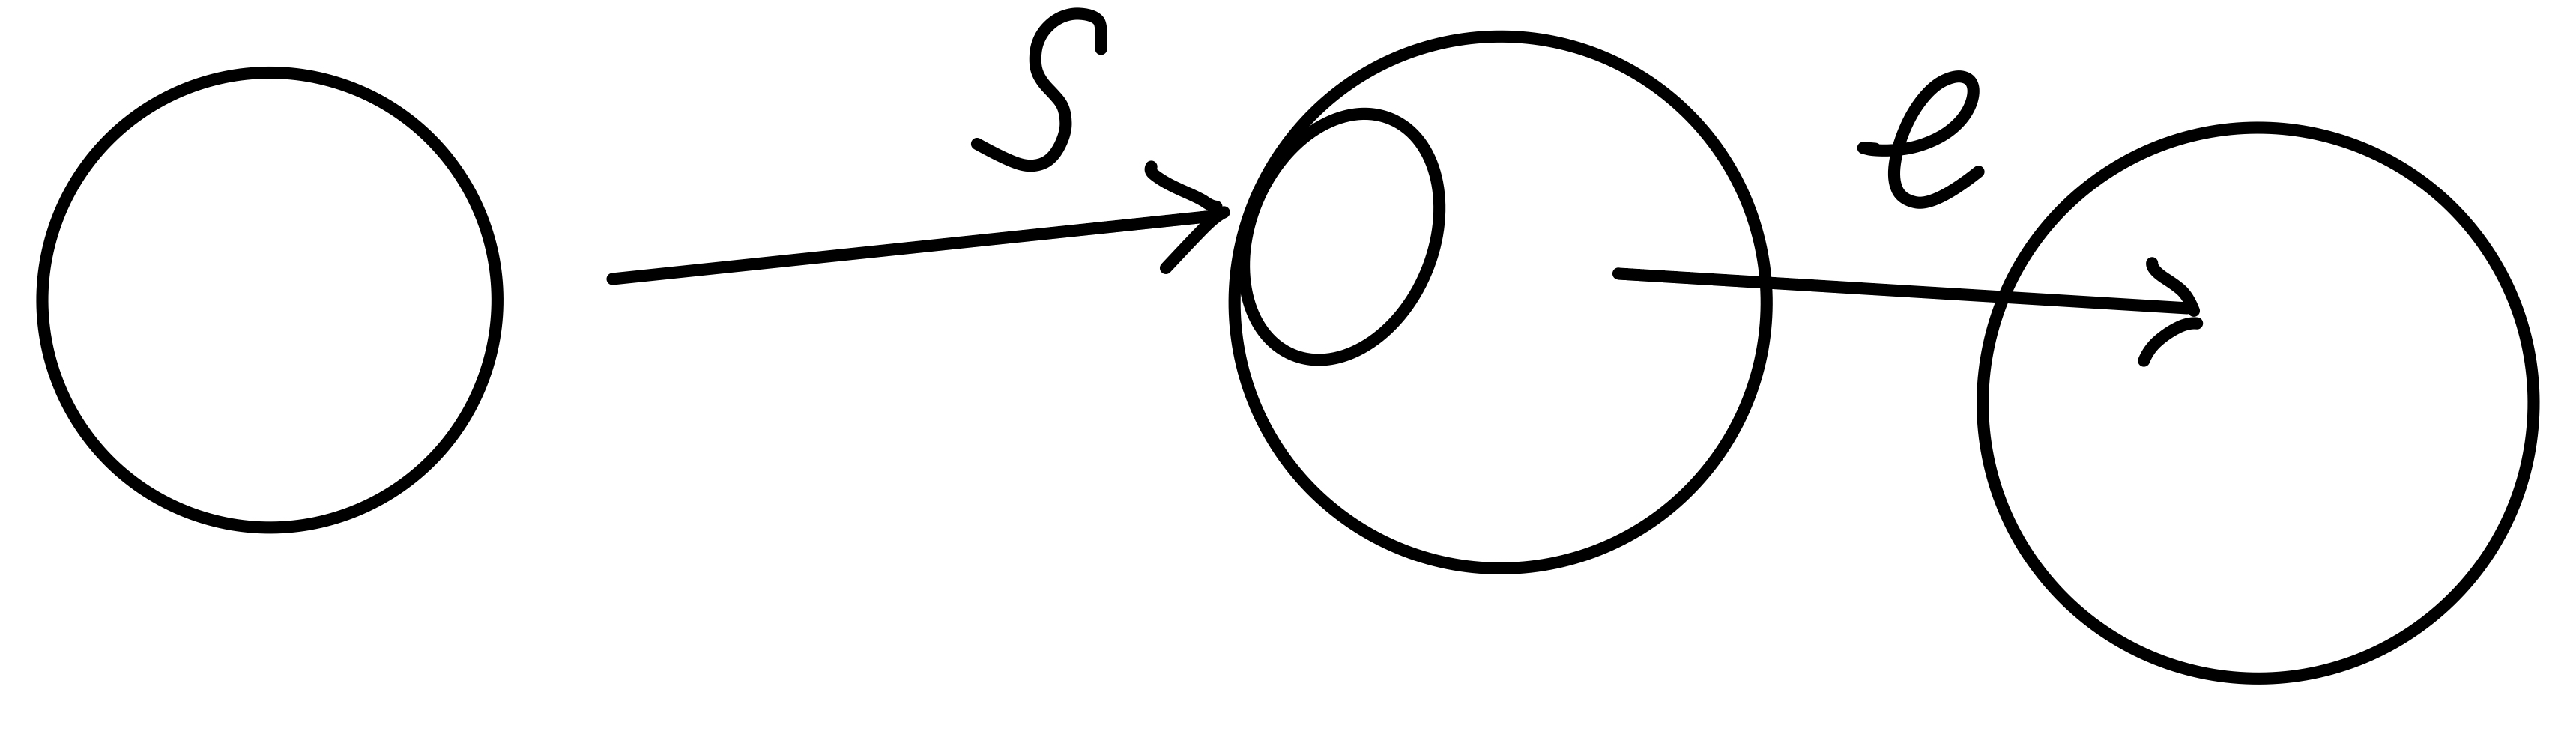
\includegraphics[width=0.4\textwidth]{figures/2FC91310-FBF1-4D04-ABDB-24F1FDF8893A}
    \caption{Schema.}
    \label{fig:2fc91310-fbf1-4d04-abdb-24f1fdf8893a}
\end{figure}

Our one-way functions will typically possess the following properties:
\begin{itemize}
    \item \textbf{Length-regularity:} $|x| = |y| \implies |f(x)| = |f(y)|$ (commonly holds),
    \item \textbf{Length-preservation:} $|f(x)| = |x|$ (sometimes holds),
    \item \textbf{Length-poly-boundedness:} $|x|^{\Omega(1)} \leq |f(x)| \leq |x|^{O(1)}$ (always holds),
    \item Not necessarily defined on each length,
    \item Can be suitably partitioned into slices.
\end{itemize}

\begin{exercise}
    Consider the existence of the following:
    \begin{itemize}
        \item one-way functions,
        \item one-way functions with the above properties,
        \item families of one-way functions.
    \end{itemize}
    Determine what is equivalent, what is not, and what remains unclear.
    Note that a family contains more than one pair $(s_n, e_n)$ for each $n$.
\end{exercise}
\begin{proof}
	Hint: when owf has a sampler $s$, hence it works good only on sampler strings.
	One can get rid of sampler by using a composition of the function with the sampler itself:  $f(r) = e(s(r))$.
	Also, when one wants to get rid of the generator $G$, then random bits of $G$ can be included as arguments for a new function.
\end{proof}

\begin{definition}
    A \emph{strong one-way function (OWF)} is an OWF such that, for all $k$, an adversary cannot achieve a success probability greater than $\frac{1}{n^k}$.

    \emph{Weak one-way functions (OWFs)} are those for which there exists a constant $k$ such that an adversary cannot achieve a success probability greater than $1 - \frac{1}{n^{k}}$.
\end{definition}

\begin{theorem}
    Each weak one-way function (OWF) can be transformed into a strong OWF.
\end{theorem}

\begin{proof}
    Let $f_w$ be a weak OWF.
    Define the function
    \[
        f_s(x_1, \ldots, x_m) = (f_w(x_1), \ldots, f_w(x_m)),
    \]
    where $m = m(n) = \Omega(n)$ is some polynomial.

    Assume there exists an adversary $A_s$ that inverts $f_s$ with probability at least $\frac{1}{n^{k_s}}$.
    We will construct an adversary $A_w$ that breaks $f_w$.
    
    The construction of $A'_w(y)$ is as follows:
    \begin{itemize}
        \item For each $j \in [m]$,
        \item Select $x_1, \ldots, x_m$ uniformly at random,
        \item Let $x = A_s(f_w(x_1), \ldots, f_w(x_{j - 1}), y, f_w(x_{j + 1}), \ldots, f_w(x_m))_j$,
        \item If $f_w(x) = y$, return $x$.
    \end{itemize}
    
    Finally, $A_w$ repeats $A'_w(y)$ for $a(n) = \poly(n)$ times and returns the most frequently occurring result.
    The precise choice of $a(n)$, a suitable polynomial, will be determined later.

    Let $S$ denote the success set for $A'_w$:
    \[
        S = \left\{y \in \{0, 1\}^n \mid \Pr[A'_w \text{ inverts } f_w \text{ on } y] > \frac{n}{a(n)}\right\}.
    \]
    The overall success probability of $A_w$ is then at least
    \begin{align*}
        \Pr[y \in S] &\cdot \underbrace{\Pr[A_w \text{ inverts } f_w \text{ on } y \mid y \in S]}_{1 - (1 - \frac{n}{a(n)})^{a(n)}}\\
					 &= \Pr[y \in S] \cdot \left( 1 - \left(\left( 1 - \frac{1}{a(n) / n} \right)^{a(n) / n}\right)^{n}  \right) \\
					 &\approx \Pr[y \in S] \cdot \left(1 - \frac{1}{e^n}\right).
    \end{align*}

    \begin{claim}
        $\Pr[y \in S] \geq 1 - \frac{n}{m}$, where $m$ is the number of copies.
    \end{claim}
    
    \begin{proof}
        Assume that $\Pr[y \in S] < 1 - \frac{n}{m}$.
        Then,
        \[
            \Pr[A_s \text{ succeeds}] \leq \Pr[x_i \in S, \; \forall i \in [m]] + \Pr[\text{success if not all in } S].
        \]
        \begin{itemize}
            \item Since $\Pr[y \in S] < 1 - \frac{n}{m}$, we have 
            \[
                \text{All in } S \leq \left( 1 - \frac{n}{m} \right)^{m}  = \left(\left(1 - \frac{1}{m/n}\right)^{m/n}\right)^n \approx \frac{1}{e^n}.
            \]
            \item If not all $x_i$ are in $S$, then the probability of success is at most $\frac{n}{a(n)} \cdot m$, as we assume none of the $x_i$ are in $S$.
        \end{itemize}
        Therefore, the sum of these probabilities is at most
        \[
            \frac{1}{e^{n}} + \frac{n}{a(n)} \cdot m.
        \]
        By choosing $a(n)$ sufficiently larger than $m$, it follows that $A_s$ does not successfully invert $f_s$.
    \end{proof}

    Using this claim, we conclude that the success probability of $A_w$ is at least
    \[
        \Pr[y \in S] \cdot \left(1 - \frac{1}{e^{n}}\right) \ge \left(1 - \frac{n}{m}\right) \cdot \left(1 - \frac{1}{e^{n}}\right).
    \]
\end{proof}

\begin{example}
    Let $f(a, b) = a \cdot b$.
    This function can often be inverted due to the fact that $a \cdot b$ is typically divisible by~two.
\end{example}

\begin{example}
    Let $f(p, q) = p \cdot q$, where $p, q \in \mathbb{P}$, $p < q$, and $\log p \approx \log q$.
\end{example}

\begin{example}
    Define the function
    \[
        f(x_1, \ldots, x_n, I) = (x_1, x_2, \ldots, x_n, \sum_{i \in I} x_i),
    \]
    where $I \subseteq [n]$.
	This corresponds to the \emph{Subset Sum} problem, which is $\NP$-complete.
\end{example}

\begin{example}[Discrete logarithm]
    Take $p \in \mathbb{P}$.
    Let $g$ be a generator in $\mathbb{F}_p$, and consider $x \in \mathbb{Z}_{p - 1}$.
    Define
    \[
        f(x) = g^x \mod p.
    \]
    This function is called a logarithm because, to invert it, one must find $\log_g(g^x)$.
\end{example}

\begin{definition}
    We say that $f$ can be reduced to $g$ (denoted $f \to g$) if there exists a randomized polynomial-time algorithm $T^{\bullet}$ such that, for all values of $k_f$, there exists a corresponding $k_g$ satisfying the following condition:
    For any adversary $A$, if $A$ inverts $g$ with probability at least $1 - \frac{1}{n^{k_g}}$, then there is an algorithm $T^A$ that inverts $f$ with probability at least $1 - \frac{1}{n^{k_f}}$.
\end{definition}

\begin{theorem}[Universal one-way function]
    There exists a \emph{universal} weak one-way function $u$ such that for all $f \in \fP$, we have $f \to u$.
\end{theorem}

\begin{proof}
    Define $u(M, x) = (M, M(x))$, where $x \in \{0, 1\}^*$ and $M$ is a description of a Turing machine.
    Here, $M(x)$ denotes the output of $M$ on input $x$ within $|x|^2$ steps (to ensure that $u$ is computable).

    \begin{lemma}
        Without loss of generality, a weak OWF $f$ is computable within $|x|^2$ steps.
    \end{lemma}
    
    \begin{proof}
        Define an extended function $\tilde{f}(x_1, x_2) = f(x_1) \circ x_2$, where $|x_1| = n$ and $|x_2| = m = m(n)$.
        Choose $m(n)$ such that $(|x_1| + |x_2|)^2$ steps suffice to compute $f(x_1) \circ x_2$.
    \end{proof}

    Let $M^*$ be a Turing machine that computes the fixed function $f$.
    Then $u(M^*, x)$ computes $M^*(x)$ for a fraction $\mu = \frac{1}{2^{O(|M^{*}|)}} = \const$ of inputs.
    Therefore, if we invert all but a fraction of $\frac{1}{n^{k}}$ of $u$'s inputs, we can also invert sufficiently many inputs of the form $u(M^*, x)$, specifically, at least a fraction of $\mu - \frac{1}{n^{k}}$, which corresponds to $v = 1 - \frac{1}{\mu n^{k}}$ in terms of $M^*$ on inputs of length $n - |M^*|$.
    Thus, we can invert $f$.
\end{proof}

\begin{exercise}
    Consider the case of a strong one-way function (OWF).
    How does the analysis differ in this context?
\end{exercise}
\begin{proof}
	Hint: you need to use also another result from the lecture.
\end{proof}

\begin{exercise}
    What about deterministic or non-uniform adversaries?
\end{exercise}

\subsection{Trapdoor function}

We now define a function that can be inverted by its creator, yet remains infeasible to invert for others.

\begin{definition}
    A \emph{trapdoor function family (TDFF)} is a collection of polynomial-time functions $e_n$ and $d_n$ such that $d_n(e_n(x)) = x$, and for any adversary $A$,
    \[
        \Pr[A \text{ inverts } e_n \text{ on } x] \text{ is negligible}.
    \]
\end{definition}

The challenge lies in the fact that there is no uniform algorithm $D(n, x)$ for computing $d_n$, as $d_n$ is not invertible in polynomial time. A more precise definition follows.

\begin{definition}
    A TDFF is a deterministic polynomial-time algorithm $G \colon (1^n, r_g) \to (e, d, s)$ that generates Boolean circuits with the following properties:
    \begin{itemize}
        \item $e \colon \{0, 1\}^n \to \{0, 1\}^{s(n)}$ (the encryptor),
        \item $d \colon \{0, 1\}^{s(n)} \to \{0, 1\}^n$ (the decryptor),
        \item $s \colon \{0, 1\}^{\sigma(n)} \to \{0, 1\}$ (a sampler).
    \end{itemize}
    These satisfy the property that, for all $x \in \text{Im}(s)$, we have $d(e(x)) = x$. Moreover, for every adversary $A$ and for every $k \in \mathbb{N}$, there exists an $N$ such that for all $n > N$,
    \[
        \Pr[A(e(s(r_s)), 1^n, e, s) \in e^{-1}(e(s(r_s)))] < \frac{1}{n^k},
    \]
    where $G(1^n, r_g) = (e, d, s)$, and $\Pr$ is taken over the randomness of $A$ and the uniformly distributed $r_g$ and $r_s$.
\end{definition}

Essentially, the main difficulty arises from the randomness in the bits.
Given $e$ and knowledge of the specific bits used, inversion is feasible (as $d$ can be generated).
However, without knowledge of these bits, inversion becomes computationally challenging.

\begin{example}[RSA, Rivest-Shamir-Adleman]
    Let $p, q \in \mathbb{P}$ (secret).
    Define $N = p \cdot q$ (publicly known).
    Choose $\epsilon, \delta$ from $\mathbb{Z}_N$ such that $\epsilon \cdot \delta = 1 \mod (p - 1)(q - 1)$ (secret).
    Then define $s(x) = x$, $e(x) = x^{\epsilon} \mod N$, and $d(x) = x^{\delta} \mod N$.
\end{example}

\begin{proof}
    We show that this construction works:
    \[
        d(e(x)) = x^{\epsilon \delta} \mod N = x \mod N,
    \]
    by Fermat's Little Theorem.
\end{proof}
